\section{Kiến trúc hệ thống}

\subsection{Domain Driven Design}

\begin{frame}{Domain Driven Design là gì}
	\alert{Domain-Driven Design} là một phương pháp trong việc phân tích và phát triển phần mềm trong khi giải quyết nghiệp vụ phức tạp. Ý tưởng của cách thức này là xây dựng sự kết nối chặt chẽ giữa thiết kế phần mềm và mô hình nghiệp vụ.
\end{frame}

% \begin{frame}{Ba nguyên tắc}
% 	\begin{itemize}
% 		\item Trọng tâm của dự án là những nguyên tắc và logic nghiệp vụ
% 		\item Cách thiết kế phức tạp dựa trên các mô hình nghiệp vụ.
% 		\item Sự hợp tác giữa các chuyên gia kỹ thuật và miền là rất quan trọng để tạo ra một mô hình ứng dụng giải quyết các vấn đề cụ thể trong mô hình nghiệp vụ.
% 	\end{itemize}
% \end{frame}

% \begin{frame}{Đa tầng}
% 	\begin{description}
% 		\item[Tầng Application] Không chứa logic nghiệp vụ, dẫn dắt người dùng bởi các giao diện
% 		\item[Tầng Domain] Chứa khái niệm về nghiệp vụ, chỉ nằm ở trung tâm, tách biệt với các tầng khác
% 		\item[Tầng Infrastructure] Làm việc trực tiếp với hạ tầng và cơ sở dữ liệu
% 	\end{description}
% \end{frame}

\begin{frame}{Khuôn mẫu}
	\begin{description}
		\item[Entity] Các đối tượng được định danh
		\item[Value Object] Mô tả các khía cạnh của domain, bất biến, không có định danh
		\item[Aggregate] Nhóm các Entity và Value Object, đảm bảo toàn vẹn và ràng buộc
		\item[Service] Interface của hành động, chỉ quan tâm đến đối tượng xử lý bởi Service
		\item[Repository] Nơi lưu trữ đối tượng, dùng để truy xuất toàn cục
	\end{description}
\end{frame}

% \subsection{Onion}
%
% \begin{frame}{Kiến trúc Onion}
% 	\alert{Kiến trúc Onion} được xây dựng trên mô hình nghiệp vụ trong đó các lớp được kết nối thông qua các interface. Ý tưởng là giữ các phụ thuộc bên ngoài càng xa càng tốt, nơi các thực thể nghiệp vụ và các quy tắc nghiệp vụ tạo thành phần cốt lõi của kiến trúc.
% \end{frame}
%
% \begin{frame}{Ưu điểm}
% 	\begin{itemize}
% 		\item Nó cung cấp kiến trúc linh hoạt, bền vững và dễ mở rộng
% 		\item Các lớp được liên kết chặt chẽ và có sự phân tách rõ ràng
% 		\item Nó cung cấp khả năng bảo trì tốt hơn vì tất cả mã code phụ thuộc vào các lớp sâu hơn hoặc lớp trung tâm
% 		\item Cải thiện khả năng kiểm tra vì các kiểm tra có thể được tạo cho các lớp riêng biệt mà không ảnh hưởng đến các lớp khác
% 		\item Các công nghệ có thể dễ dàng thay đổi mà không ảnh hưởng đến nghiệp vụ lõi
% 	\end{itemize}
% \end{frame}
%
% \begin{frame}{Nguyên lý}
% 	\begin{description}
% 		\item[Sự phụ thuộc] Các lớp bên ngoài phụ thuộc vào các lớp bên trong và các lớp bên trong hoàn toàn không nhận biết được các lớp bên ngoài
% 		\item[Bao bọc dữ liệu] Mỗi lớp bao bọc hoặc ẩn các chi tiết triển khai bên trong và cung cấp API cho lớp bên ngoài
% 		\item[Tách mối quan tâm] Ứng dụng được chia thành các lớp trong đó mỗi lớp có một tập hợp các trách nhiệm và giải quyết các mối quan tâm riêng biệt
% 		\item[Rằng buộc] Rằng buộc thấp trong đó một module tương tác với một module khác và không cần quan tâm đến các phần bên trong của module đó
% 	\end{description}
% \end{frame}

\subsection{Hệ thống Backend}

\begin{frame}{Thành phần hệ thống Backend}
	\begin{description}
		\item[Service] Là thành phần đảm nghiệm hệ thống HTTP, xử lý các truy cập từ Frontend
		\item[Storage] Là thành phần tổng hợp dữ liệu, thực hiện A/B Test cho tầng Service
		\item[Database] Là thành phần quản lý dữ liệu cho tầng Storage
		\item[Types] Tổng hợp các thực thể ở tầng Backend
	\end{description}
\end{frame}

% \begin{frame}{Hệ thống API}
% 	\begin{table}
% 		\centering
% 		\begin{tabular}{|l|l|}
% 			\hline
% 			\textbf{Đường dẫn} & \textbf{Chú thích}                          \\ \hline
% 			/summary           & Gọi toàn bộ thông tin của hệ thống A/B Test \\ \hline
% 			/abtest            & Thực hiện A/B Test                          \\ \hline
% 			/product/create    & Khởi tạo Product mới                        \\ \hline
% 			/product/update    & Cập nhật Product                            \\ \hline
% 			/layer/create      & Khởi tạo Layer mới                          \\ \hline
% 			/layer/update      & Cập nhật Layer                              \\ \hline
% 			/exp/create        & Khởi tạo Experiment mới                     \\ \hline
% 			/exp/update        & Cập nhật Experiment                         \\ \hline
% 			/group/create      & Khởi tạo Test Group mới                     \\ \hline
% 			/group/update      & Cập nhật Test Group mới                     \\ \hline
% 		\end{tabular}
% 	\end{table}
% \end{frame}

\subsection{Biểu đồ tuần tự}

\begin{frame}{Khởi tạo A/B Test}
	\begin{figure}
		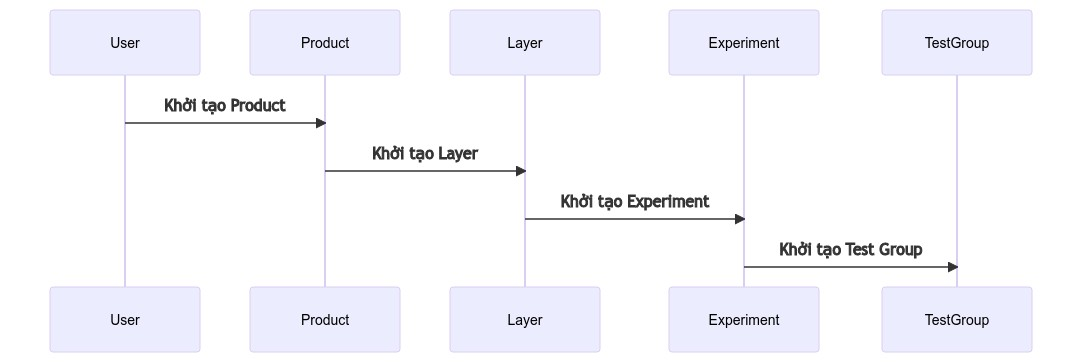
\includegraphics[width = 1\textwidth]{abtest-sequence}
	\end{figure}
\end{frame}

\begin{frame}{Thực hiện A/B Test}
	\begin{figure}
		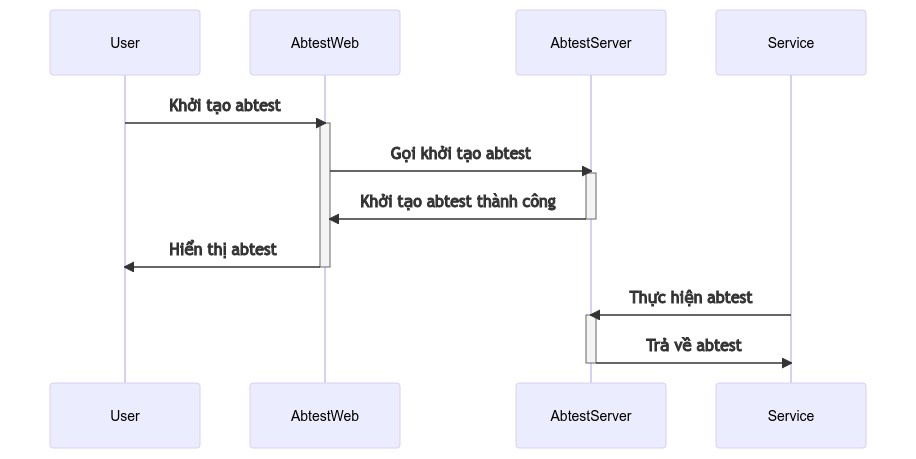
\includegraphics[width = 1\textwidth]{overview-sequence}
	\end{figure}
\end{frame}
